\documentclass[a4paper,12pt]{article}
   % Packages and definitions:
   % {
      \usepackage{a4wide}
      \usepackage{float}
      \usepackage[swedish,english]{babel}
      \usepackage[utf8]{inputenc}
      \usepackage{amsmath}
      \usepackage{amssymb}
      \usepackage{color}
      \usepackage{lipsum}
      \usepackage[backend=bibtex,style=numeric-comp,sorting=none]{biblatex}
      \bibliography{papers}
      \usepackage{subcaption}
      \usepackage[font={small}]{caption}
      \usepackage{booktabs}
      \usepackage{tikz}
      \usetikzlibrary{decorations, matrix, arrows, shapes, positioning, calc, fit}
      \tikzset{
         mybox/.style={draw, minimum height=.8cm, minimum width=.9cm},
         myflip/.style={draw, fill=gray!30, minimum height=.8cm, minimum width=.9cm},
         myint/.style={draw, minimum height=.8cm, minimum width=1.1cm},
         mynone/.style={draw=none}
      }
      \usepackage{graphicx,epstopdf}
      \epstopdfsetup{update} % only regenerate pdf files when eps file is newer
      \usepackage{cleveref}
      \usepackage{collcell} % loads array
      \newcolumntype{m}{>{$} r <{$}}
      \newcolumntype{u}{>{$[\collectcell\si} l <{\endcollectcell]$}}
      \newcommand{\approxtext}[1]{\ensuremath{\stackrel{\text{#1}}{=}}}
      \newcommand{\matr}[1]{\mathbf{#1}}
      \newcommand{\partt}[2]{\ensuremath{\dfrac{\partial {#1}}{\partial {#2}}}}
      \renewcommand{\d}[1]{\ensuremath{\operatorname{d}\!{#1}}} % non-italized differentials
      \newcommand{\h}[0]{\ensuremath{\hbar}} % hbar
      \newcommand{\qed}[0]{\ensuremath{\tag*{$\square$}}} % QED square
      \def\changemargin#1#2{\list{}{\rightmargin#2\leftmargin#1}\item[]}
      \let\endchangemargin=\endlist 
      \usepackage{amsthm}
      \theoremstyle{plain}
      \newtheorem{thm}{theorem} % reset theorem numbering for each chapter
      \theoremstyle{definition}
      \newtheorem{defn}[thm]{definition} % definition numbers are dependent on theorem numbers
      \newtheorem{exmp}[thm]{example} % same for example numbers
      \renewcommand{\theequation}{\thesection.\arabic{equation}}
      \def\changemargin#1#2{\list{}{\rightmargin#2\leftmargin#1}\item[]}
      \let\endchangemargin=\endlist    
      \newcommand{\ts}{\textsuperscript} 
   % }
\title
{
	\textbf
	{
      Linking the Dynamics of Genetic Algorithms to the Encoding of Information
   }\\[1em]
}

\author{Henrik Åhl}
   \date{\today}

\begin{document}
\begin{titlepage}
   \begin{flushright}
   LU TP 16-29\\
   June 2016\\
   \end{flushright}
   \vfill
   
   \begin{center}
      {\large\bf LINKING THE DYNAMICS OF GENETIC ALGORITHMS TO THE ENCODING OF
      INFORMATION\\[3mm]
      Bachelor's thesis}
      \\[3cm]
      {\bf Henrik Åhl}
      \\[5mm]
		{Department of Astronomy and Theoretical Physics, Lund University}
		\\[2cm]
		{Thesis supervised by Carl Troein and Adriaan Merlevede}
		\vfill
		% use the eps version for latex and the pdf version for pdflatex 
		\includegraphics[height=4cm]{logocLUeng.pdf}
	\end{center}
	\thispagestyle{empty} % do not count pages just yet
\end{titlepage}
   \pagebreak
   \thispagestyle{empty} % do not count pages just yet
   \phantom{p\\[5cm]}
   \vfill
\begin{otherlanguage}{swedish}
   \noindent\textit{Wisely and slow; they stumble that run fast.\\[1em]
--- Friar Lawrence, to Romeo}
\end{otherlanguage}
\vfill
   \pagebreak
   \phantom{p}
\begin{abstract}
      \noindent Genetic algorithms are complex constructs often used as heuristic search
      methods in contexts ranging from combinatorial optimisation to
      \textit{in silico} evolution. They draw inspiration from the 
      principles of biological evolution by utilizing the concepts of mutation,
      reproduction and selection in order to improve a population of solutions. 
      The solutions are often represented as abstract data sequences, e.g.\ as
      binary strings, though it has been shown that the choice of
      encoding alters the performance of the search. 

      In this thesis, the dynamics of four types of encodings used to evolve a set
      of integers are investigated: the previously researched bijective
      \textit{Binary} and 
      \textit{Gray code} maps, as well as an introduced encoding scheme which includes
      non-coding data, denominated the \textit{consensus} map. Coding parts
      of the consensus sequences are signified by pre-determined start sequences,
      after which subsequent code is interpreted via either the Binary or the Gray code 
      scheme. 
      
      The performance of the genetic algorithm is measured by the ability 
      to solve four problems with different search spaces. The dynamics are also investigated by 
      identifying the effects the encodings have on the distribution of cost
      effects due to point mutations, as well as by the ability to produce good
      solutions under a range of different mutation rates.
      
      It is found that the bijective maps give rise to similar distributions of
      cost effects, but significantly different performances. The consensus encodings 
      instead allow for higher robustness with respect to different mutation
      rates, as well as a robustness towards highly negative effects due to
      point mutations. It is also shown that having an
      encoding--decoding map which allows for both smaller and larger steps in 
      phenotype-space is an important part of being able to produce good
      solutions in a range of cases. 
\end{abstract}
\vfill
	\thispagestyle{empty} % do not count pages just yet
\newpage
\section*{Populärvetenskaplig sammanfattning}
\begin{otherlanguage}{swedish}
   \thispagestyle{empty} % do not count pages just yet
   \textit{Genetiska algoritmer} utgör en grupp sökalgoritmer som
   hämtar inspiration från evolutionära processer i biologiska sammanhang. Genom
   att låta \textit{populationer} av enskilda datasekvenser, exempelvis strängar av
   ettor och nollor, representera olika
   lösningar till ett givet problem, och sedan successivt låta datasekvenserna
   utbyta information sinsemellan, samt att genom mutationer modifiera dem, är det möjligt att 
   producera optimala eller väldigt goda lösningar till problemet i fråga; allt 
   som principiellt behövs är ett sätt att \textit{tolka} en datasekvens och ett sätt 
   att \textit{utvärdera} hur bra eller dålig den i sammanhanget är. Populationer
   kan också växa, reduceras eller förändras innehållsmässigt över tidssteg -- så
   kallade \textit{generationer} -- under sökningen.
   Vanligtvis ges populationsmedlemmar som utvärderats som bättre lösningar än
   andra större utrymme att föröka sig eller överleva, så att en partiskhet gentemot
   högpresterande datasekvenser förekommer, i enlighet med selektionstrycket
   inom just biologisk evolution.

   På så vis skiljer sig genetiska algoritmer från många andra sökalgoritmer, 
   som istället ofta använder sig av direkt matematiska metoder för att hitta 
   bättre lösningar. Detta gör dem i synnerhet lämpliga för problem där det inte existerar någon
   direkt bakomliggande matematisk konstruktion, eller då det är ovanligt
   svårt att formulera den. De stora likheterna med biologisk evolution medför
   också att genetiska algoritmer kan användas som verktyg för att förstå just
   evolutionära processer, som ofta är oerhört komplexa och icke-intuitiva. 

   Det har dock visat sig att hur en lösning utläses från en datasekvens --
   eller motsvarande, hur informationen i sekvensen är inkodad -- spelar
   roll för hur väl algoritmen presterar. Olika typer av informationsinkodningar
   medför också olika typer av evolutionär dynamik, vilket har konsekvenser för på
   vilket sätt populationen av lösningar successivt blir bättre. 
   
   För att ytterligare förstå på vilket sätt inkodningen är av vikt, och vilken sorts
   dynamik som medföljer en viss representation av information, undersöks i
   denna uppsats olika inkodningar och konsekvenserna som dessa får för
   mutationseffekter på datasekvenserna. Att i högre 
   grad förstå denna komplexa dynamik kan i slutändan förhoppningsvis medföra en djupare 
   förståelse för funktionerna hos genetiska strängar i framför allt datavetenskapliga
   sammanhang, men också hos deras motparter i naturen.
\end{otherlanguage}
\newpage
   \thispagestyle{empty} 
   \tableofcontents
\newpage
\setcounter{page}{1}
\section{Background}
   \subsection{The study of genetic algorithms}
      \textit{Genetic algorithms} (GAs) make up a family of computational models inspired
      by the evolutionary principle of natural selection. They are used as population-based 
      heuristic search methods, and provide wide 
      applications for problems related to especially computational and
      combinatorial optimisation. 
      Because of the similarities to biological evolution, they are also, along with
      other methods adhering to the principles of \textit{Evolutionary
      computation}, such as \textit{Evolutionary algorithms, Genetic
      programming} and \textit{Evolution strategies}, occasionally also used to study 
      the dynamics of evolutionary processes~\cite{sudoku}. However, because
      many of the methods are principally alike, the
      distinction of what strictly defines GAs is often unclear, but they can in
      broader terms be viewed as all 
      population based models which utilize \textit{selection}, \textit{recombination} and \textit{mutation}
      operators to produce sample points in a search space. These three pillars of GAs are often referred to
      as \textit{genetic operators}~\cite{tutorial}.

      Implementations of GAs typically feature information encoded
      as a population of strings of bits, although also real-valued and
      non-binary encodings are common for solving many
      problems~\cite{virtual_alphabets,real_coded_goldberg}. 
      The encoded information, denoted the \textit{genotype}, serves as an
      abstraction of a candidate solution, normally referred to as the
      \textit{phenotype}. Phenotypes are evaluated by a performance
      measuring function, such as a \textit{fitness}, \textit{cost} or
      \textit{objective} function, which are all in principle equivalent, but are usually used to
      signify different measures. For example, the cost function stands as the
      opposite of fitness, i.e.\ as fitness increases, the cost decreases. The
      objective function is similarly simply a name for the measure of the
      ability to solve some specified objective. 
      
 %    Regardless of which approach is used in a given situation,
      Especially in optimisation settings, the strength of GAs often come from their lack of need of a 
      derivative in order to traverse the search space. Instead, change and successive
      progression is determined by the genetic operators, which generate new
      points based on the previous state.  
      Compared to other gradient-less global search methods, such as
      \textit{simulated annealing}, GAs have been proven to perform
      better in certain cases of combinatorial optimisation, such as component
      placement in electric circuits, as shown by Manikas
      and Cain~\cite{ga_vs_sa}, as well as in telecommunications traffic
      routing, which Mann and Smith~\cite{Man96} demonstrated. On the other hand, Jennison and
      Sheehan~\cite{ga_bad} propose that GAs typically are not well suited for solving 
      computational optimisation problems with large sets of variables of equal significance. 
         
      In settings which instead aim to investigate the dynamics of evolutionary
      systems, GAs, due to their similarities with the process of natural evolution, 
      provide a natural approach for investigating various features of evolutionary
      behaviour. The systems investigated are not necessarily required to be biological, as
      they have been used in order to understand, among many other things, the evolution 
      of grammar, communication, age preference between sexes, and evolvability
      itself~\cite{grammatical_evolution,
      evol_of_communication,
      evol_of_female_preference,
      evol_of_evol,evol_of_evol_in_gp}. 
      Hu and Yang~\cite{sudoku} additionally utilize GAs as tools to understand sequence 
      evolution under constraints by solving the game of Sudoku. The underlying structure and theory of the genotype--phenotype map, which
      is often applied to understand GAs, has also been studied in other contexts, 
      as by Stadler et al.~\cite{topology_of_the_possible} 
      when questioning the current view of the link between the genotype and
      the phenotype space.  In relation to this, it has been shown that how one 
      encodes information, i.e.\ the phenotype, can be of importance for how well 
      the algorithms perform. As GAs traverse a search space of possible solutions with
      varying fitness, i.e.\ a \textit{fitness landscape}, the encoding of 
      information is a determining factor for the shape of the landscape.
      Consequently, the encoding affects the ability of the GA to traverse
      different states and thus also the capability of finding the global
      optimum~\cite{transforming_the_ss_with_gray}.
      
      However, even though GAs have been a subject of interest for many years,
      and featured a wide range of applications within various fields of
      science and engineering, their dynamics have not been thoroughly
      investigated. In this thesis it is therefore analysed
      how the encoding of information alters the ability of
      GAs to solve problems of different complexities. It
      has previously been proposed that the encoding should preferably be bijective in the sense
      that the genotype--phenotype map should have a one-to-one
      link~\cite{intro_to_evol_alg, tutorial}; a proposition here investigated
      further by the introduction of encodings including ``dead code'', which
      has no direct effect on the phenotype, but instead allows for increased phenotypic accessibility
      and alternative evolutionary pathways. The effects which neutral encodings
      have on the search process have previously been demonstrated by Shipman et al.\
      \cite{Shipman2000}, but the fitness effects due to operations on encodings providing 
      multiple-to-one genotype--phenotype maps remain to be investigated, and could possibly
      shed further light on the dynamical aspects of these types of
      encodings. 

      The analysis is performed by investigating the distribution of fitness effects 
      due to point mutations on the genotype, as well as by evaluating performances 
      with respect to the ability to solve specific problems with varying
      complexity. The encodings are also examined by their ability to produce
      good solutions for a range of mutation rates.   

   \subsection{General structure}
      \subsubsection{From code to fitness}
      How a GA is structured varies greatly on a case by case basis. This is
      largely due to the \textit{No Free Lunch Theorem}, which states that no
      general purpose optimisation strategy can be optimal for all 
      problems~\cite{no_free_lunch}. Consequently, a wide variety
      of GAs exist, where the specific implementations depend 
      on what exact tasks the algorithms are applied to. Regardless, a general structure can still be established.

      %% GENOTYPE %%
      As stated, GAs are population-based in the sense that a set of candidate solutions 
      are maintained during execution. The genotypes, which are also known as 
      \textit{chromosomes} or \textit{genomes}, are typically encoded as a string of bits 
      or real-valued numbers, but occasionally also as other types of data structures~\cite[p.\ 60--82]{Goldberg_GA_book}. 
      The genotype sequence can be of either fixed or variable
      length, although fixed length genomes are far more prevalent~\cite{varlen,varlen2}.
      
      Genomes normally code for homologous types of information in
      subsections referred to as \textit{genes}. For example, in a
      parameter optimisation setting, the individual genes can be chosen to code
      for separate parameters in an equation. Variations of GAs
      with heterogeneously encoded parameters, i.e.\ parameters of different,
      non-compatible types, within a single chromosome do, however, also exist~\cite{HELGA}. 

      %% PHENOTYPE TO FITNESS %%
      Each individual genotype in the population has to be interpreted via an 
      encoding--decoding map, or equivalently, genotype--phenotype map, in order 
      for a solution to be evaluated. In imitation of how
      phenotypes in nature fare differently due to environmental factors, the 
      phenotype is evaluated by a fitness, cost, or objective function,
      which measures how good a solution ultimately is. An example of the link between the
      genotype--phenotype--fitness stages is illustrated in~\Cref{fig:genotype_to_fitness}.
      Because every genotype gives rise to a phenotype, which is then given a
      fitness, the link between the genotype and fitness of a binary genome of
      fixed length can be seen as a mapping
      $\{0,1\}^N \rightarrow \mathbb{R}$, where $N$ is the number of bases,
      i.e.\ sequence elements, in the genome.
      
      \begin{figure}[H]
         \centering
           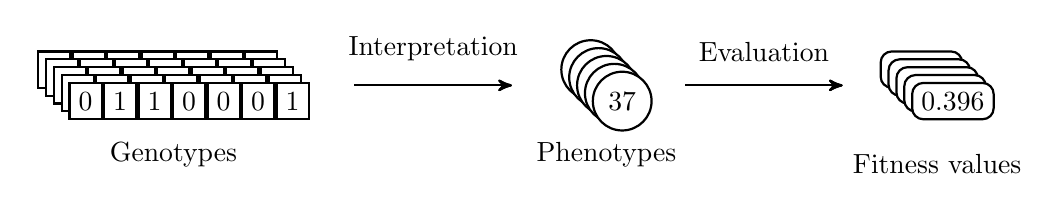
\begin{tikzpicture}[->,>=stealth',auto,
            thick,node/.style={box, draw,font=\sffamily\Large\bfseries}]
            \matrix (matrix) at (-10.0,-.0)[
                matrix of nodes,
               row 1/.style={every node/.append style={draw,fill=white,minimum width=.5em, minimum height=.4em}},
            ]{
              0  & 1 &  1 & 0 & 0 & 0 & 1   \\
            };
            \matrix (matrix2) at (-9.9,-.1)[
                matrix of nodes,
                row 1/.style={every node/.append style={draw,fill=white,minimum width=.5em, minimum height=.4em}},
            ]{
              0  & 1 &  1 & 0 & 0 & 0 & 1   \\
            };
            \matrix (matrix3) at (-9.8,-.2)[
                matrix of nodes,
                row 1/.style={every node/.append style={draw,fill=white,minimum width=.5em, minimum height=.4em}},
            ]{
              0  & 1 &  1 & 0 & 0 & 0 & 1   \\
            };
            \matrix (matrix4) at (-9.7,-.3)[
                matrix of nodes,
                row 1/.style={every node/.append style={draw,fill=white,minimum width=.5em, minimum height=.4em}},
            ]{
              0 & 1 &  1 & 0 & 0 & 0 & 1   \\
            };
            \matrix (matrix5) at (-9.6,-.4)[
                matrix of nodes,
                row 1/.style={every node/.append style={draw,fill=white,minimum width=.5em, minimum height=.4em}},
            ]{
              0 & 1 &  1 & 0 & 0 & 0 & 1   \\
            };

            \node [fill=none, below of=matrix3, node distance=2.5em] (init) {Genotypes};

             \tikzstyle{circ} = [draw, circle,fill=white!100, node distance=3cm,minimum height=1.5em]
             
             \node  [circ] at (-4.5,-.0) (1) {37};
             \node  [circ] at (-4.4,-.1) (2) {37};
             \node  [circ] at (-4.3,-.2) (3) {37};
             \node  [circ] at (-4.2,-.3) (4) {37};
             \node  [circ] at (-4.1,-.4) (5) {37};
             
             \node [fill=none, below of=3, node distance=2.5em] (pheno) {Phenotypes};
             
             \node  [rectangle, draw,fill=white!100, rounded corners] at (-.30,-.0) (11) (fitness1) {0.396};
             \node  [rectangle, draw,fill=white!100, rounded corners] at (-.20,-.1) (21) (fitness2) {0.396};
             \node  [rectangle, draw,fill=white!100, rounded corners] at (-.10,-.2) (31) (fitness3) {0.396};
             \node  [rectangle, draw,fill=white!100, rounded corners] at (-.00,-.3) (41) (fitness4) {0.396};
             \node  [rectangle, draw,fill=white!100, rounded corners] at (+.10,-.4) (51) (fitness5) {0.396};

             \node  [fill=none, below of=fitness3] (fit) {Fitness values};
             \tikzstyle{line} = [draw, -latex']
             \draw [->] (-7.5,-.2)-- (-5.5,-.2){};
             \draw [->] (-7.5,-.2)--(-5.5,-.2) node [midway, above=.5em] (interpret) {Interpretation};
             
             \draw [->] (-3.3,-.2)--(-1.3,-.2){};
             \draw [->] (-3.3,-.2)--(-1.3,-.2) node [midway, above=.5em ] (eval) {Evaluation};
         \end{tikzpicture}
         \caption{Mapping from genotype to fitness. The genotype codes for a
         phenotype which is then evaluated by a given fitness function. The
         fitness of a population is often determined by the best phenotype, although 
         various choices can be made.} 
         \label{fig:genotype_to_fitness}
      \end{figure}

      \subsubsection{Genetic operators}
         GAs rely on three types of operators for successively
         improving a population of solutions: selection, mutation and crossover.
         These operators come in many variations, with the specific
         implementation depending on the problem at hand, as well as on the
         other settings of the GA. A conceptual interpretation of the flow of 
         operations in GAs can be seen in
         \Cref{fig:structure}, although many implementations also feature a
         selection process for which individuals
         should be chosen for mutation and crossover operations. 
         
         \begin{figure}[H]
            \centering
            % Define tikz specific styles
            \tikzstyle{block} = [rectangle, draw, fill=white!20, 
                text width=5em, text centered, rounded corners, minimum height=3.5em]
            \tikzstyle{line} = [draw, -latex'] 
            \tikzstyle{cloud} = [draw,
               ellipse,fill=gray!30, node distance=3.5cm,
            minimum height=2.5em]
                
            \begin{tikzpicture}[->,>=stealth',auto, node distance=3cm,
                thick,node/.style={box, draw,font=\sffamily\Large\bfseries}]

                % Place nodes
                \node [cloud] (init) {\begin{tabular}[H]{c}Initialization\\of population\end{tabular}};
                \node [block, right of=init, node distance=4cm] (mut) {Mutation};
                \node [block, right of=mut] (crossover) {Crossover};
                \node [block, right of=crossover] (selection) {Selection};
                \node [cloud, below of=crossover, node distance=1.7cm] (newp) {New population};

                % Draw edges
                \path [line] (init) -- (mut);
                \path [line] (mut) -- (crossover);
                \path [line] (crossover) -- (selection);
                \path [line] (selection) |- (newp);
                \path [line] (newp) -| (mut);
            \end{tikzpicture}
            % Define caption and label
            \caption{Process flow scheme of a typical Genetic Algorithm. If no
            terminating condition is invoked, the number of iterations in the
         process is indeterminate. Every pass in the loop increments the current \textit{generation}.}
            \label{fig:structure}
         \end{figure}
         
         \paragraph{Selection}
            The selection operation can be applied in several parts of the
            process: in picking out individuals for reproduction, picking
            individuals to mutate, and picking individuals for death or survival.        
            It is one of the most determining features for how the population will evolve 
            as it defines the advantages an individual will have due to a higher
            fitness than another individual in the population. It also determines 
            the degree of phenotypic diversity within the population.

            Multiple choices of selection operators exist, although a few are
            more frequently applied than others. Common choices of methods are 
            \textit{elitism}, which 
            unrestrictedly favours the strongest
            individuals; 
            \textit{roulette wheel selection}, which picks individuals with
            probabilities proportional to their fitness; and 
            \textit{tournament selection}, which picks out a random subset of the population, 
            and then chooses a number of individuals from a geometric
            distribution, with the individuals sorted by
            fitness~\cite{theory_of_ga}.
            It should be noted that whenever elitism is used, it is
            often coupled together with other
            selection methods in order to maintain the genotypic and phenotypic diversity within the
            population.

         \paragraph{Mutation}
            Mutation operators alter the genome 
            such that an alternative solution is produced. Often this is done
            while keeping the individual used as basis for the mutation unaffected.
            The process can thereby be likened to a type of asexual
            reproduction. Because of this, the terms \textit{parent} and
            \textit{offspring} are commonly used whenever new individuals are
            created from other.  
            
            Typical choices of mutation operators are operators performing 
            \textit{point mutations}, which alter the value of singular bases in
            the genome;
            \textit{insertions}, which randomly produce or copy blocks
            of genotypic information that are inserted into the genome; and 
            \textit{deletions}, which delete blocks of the genome.

            Implementations of point mutations on binary genomes typically flip every
            bit in the genome with a probability $p$, as illustrated in 
            \Cref{fig:mutation_illustration}.
            \begin{figure}[H]
               \centering
               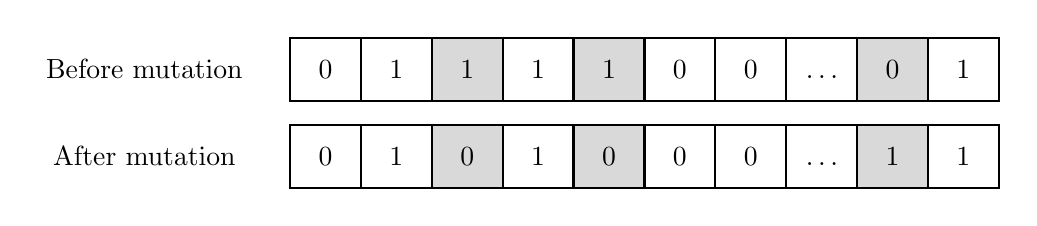
\begin{tikzpicture}[->,>=stealth',auto,
              thick,node/.style={box, draw,font=\sffamily\Large\bfseries}]
               \matrix (matrix) [
                   matrix of nodes,
                   row sep={1.1cm,between origins}, column sep=-\pgflinewidth,
                   row 1/.style={every node/.append style={mybox}},
                   row 2/.style={every node/.append style={mybox}},
               ]{
                 |[draw=none]| Before mutation\hspace{.5cm} &  0 & 1 & |[myflip]| 1 & 1 & |[myflip]| 1 & 0 & 0 & \phantom{0\hspace{-3pt}}\ldots & |[myflip]| 0 & 1   \\
                 |[draw=none]| After mutation\hspace{.5cm}  &  0 & 1 & |[myflip]| 0 & 1 & |[myflip]| 0 & 0 & 0 & \phantom{0\hspace{-3pt}}\ldots & |[myflip]| 1 & 1   \\
               };

               \end{tikzpicture}
               \caption{Example of a point mutation operation on a binary
                  genome. Bits at every index are flipped with a given
                  probability $p \in \left( 0,1 \right]$. 
                  Gray boxes show changes in the genome due to the operation.}
               \label{fig:mutation_illustration}
            \end{figure}
            
            \noindent The mutation operator can be seen as the producer of genotypic diversity within
            the population, and is the major component for sampling new points in
            the search space, which allows the algorithm to find better
            solutions~\cite{theory_of_ga}.

         \paragraph{Crossover}
            The crossover operation is the analogue of sexual
            reproduction in nature. Inspired by the recombination
            of biological chromosomes during meiosis, the process is an attempt to 
            recombine features from different genomes. 
            
            Also for crossover operators, multiple variations exist, while the most common 
            for binary genomes are single-point and dual-point crossovers, which cut the genome 
            at one or two points respectively. The resulting parts are then recombined into new
            individuals~\cite{theory_of_ga}. An illustration of a one-point
            crossover is provided in
            \Cref{fig:crossover_illustration}.

            It should be noted that a crossover operator is not strictly
            necessary for evolving GAs as mutation operators are in
            principle sufficient for sampling new points in the search space.

            \begin{figure}[H]
               \centering
               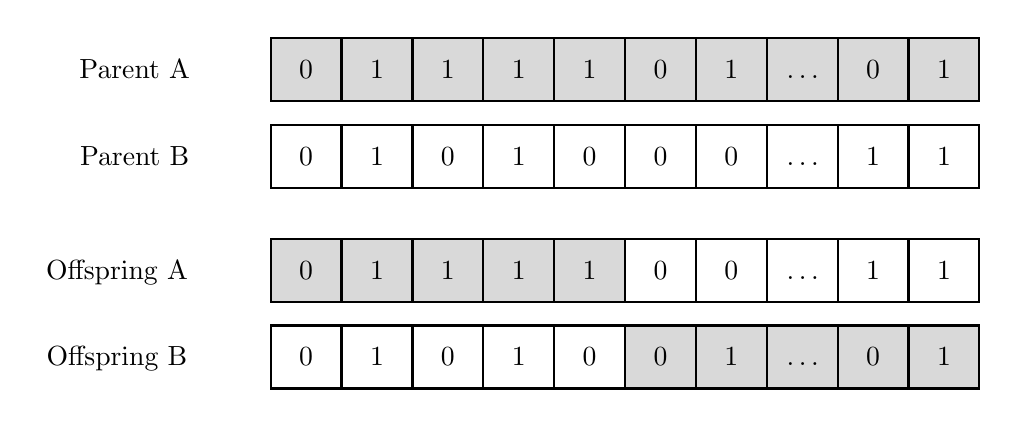
\begin{tikzpicture}[->,>=stealth',auto,
              thick,node/.style={box, draw,font=\sffamily\Large\bfseries}]
               \matrix (matrix) [
                   matrix of nodes,
                   row sep={1.1cm,between origins}, column sep=-\pgflinewidth,
                   row 1/.style={every node/.append style={myflip}},
                   row 2/.style={every node/.append style={mybox}},
                   row 3/.style={every node/.append style={myflip}},
                   row 4/.style={every node/.append style={mybox}},
               ]{
               |[draw=none, fill=white!100]| Parent A\hfill\hspace{.5cm}~&   0 & 1 & 1 & 1 & 1 & 0 & 1 & \phantom{0\hspace{-3pt}}\ldots &  0 & 1   \\
               |[draw=none]| Parent B\hfill\hspace{.5cm}~&   0 & 1 & 0 & 1 & 0 &  0 & 0 & \phantom{0\hspace{-3pt}}\ldots &  1 & 1 \\[1em]
               |[draw=none, fill=white!100]| Offspring A\hfill\hspace{0.95cm}~&  0 & 1 & 1 & 1 & 1 & |[fill=white!100]| 0 & |[fill=white!100]|0 & |[fill=white!100]|\phantom{0\hspace{-3pt}}\ldots & |[fill=white!100]| 1 & |[fill=white!100]| 1   \\
               |[draw=none, fill=white!100]| Offspring B\hfill\hspace{0.95cm}~&  0 & 1 & 0 & 1 & 0 & |[myflip]| 0 & |[myflip]| 1 & |[myflip]| \phantom{0\hspace{-3pt}}\ldots & |[myflip]|  0 & |[myflip]| 1   \\
               };
               \end{tikzpicture}
               \caption{Illustration of a one-point crossover on two parental genomes. 
                  A random or pre-chosen cutting point determines which sections of the genomes 
                  should be assigned to the corresponding offspring.}
               \label{fig:crossover_illustration}
            \end{figure}

   \subsection{The search space}
         GAs perform a search by selectively traversing 
         an $N$-dimensional search space, where $N$ is the 
         number of bases in the genome. Every configuration of the genome defines a point 
         in the search space. The population based 
         mechanism then allows for performing implicit, parallelised local search~\cite{holland,tutorial}. 
         Because the fitness is what ultimately determines whether a
         point in this search space is good or not, the fitness function is a
         defining factor of the shape of the search space. However, also the encoding 
         plays a significant role.           

      \subsubsection{The encoding of information shapes the search space}
         It has been shown that how the search 
         is performed depends largely on the encoding of information, as the encoding 
         determines the available phenotypes of a given state, and 
         thereby affects the connection between points in the fitness landscape. This implies that the 
         encoding is a significant component in how well the algorithm in turn performs on a
         particular problem~\cite{transforming_the_ss_with_gray}. 
         Because of this, the effects of the choice of encoding are in a general sense  
         inherently non-trivial to clarify. 
         However, in the specific case of encoding integers as binary strings,
         interpreting the effects on the dynamics of the GAs' temporal progression
         becomes markedly simpler. Traditionally, integers are normally encoded
         via either a
         \textit{Binary} (henceforth capitalized when referencing the encoding), or 
         a \textit{Gray code} scheme.
      
         \paragraph{Binary}
            The Binary encoding--decoding map is a straightforward and intuitive 
            way of interpreting and encoding an integer from and to a sequence 
            with a binary base. In the encoding scheme, every base value represents a 
            power of two, as is common in particular for computer-like devices. However, the Binary scheme allows for the
            existence of so-called \textit{Hamming cliffs} -- occurrences when
            two adjacent points in integer space are well separated in the
            genotype space. 
            In GAs, this can significantly hamper the
            progression of the algorithm. Consider for example the complementary
            binary strings \texttt{1000} and \texttt{0111} which in the Binary scheme
            code for the integers 8 and 7 respectively. Although these are
            adjacent in the ordered integer space, they require four bit flips in
            order to assume each other's phenotypes. This
            limitation, however, can be circumvented by the use of the Gray 
            code scheme.

         \paragraph{Gray code}
            Gray code, after its inventor Frank Gray (1887--1969), is an
            alternative way of encoding integers such that Hamming cliffs cannot
            occur. It does so by encoding integers in such a way that two adjacent
            states always lie precisely one base change away from each other,
            i.e.\ at a distance of one in genotype space.
            This simple requirement allows for the existence of multiple
            types of Gray code, which then have to be translated and interpreted
            via the Binary scheme in order to render an integer. This process makes 
            the use of Gray code less tractable and somewhat computationally
            cumbersome, but even so, 
            it has been shown that Gray code offers a significant increase in performance 
            in certain cases~\cite{transforming_the_ss_with_gray}. Like the
            Binary scheme, the Gray code map provides a bijective
            genotype--phenotype map, but Gray coded sequences are not guaranteed
            to undergo a translation in integer-space corresponding to a power of two when a
            single bit is changed.  
            
         \subsubsection{Neutral evolution}
            Literature on GAs often mentions the importance of using an
            encoding--decoding map which is bijective; usually with the argument
            that such a choice decreases the size of the search space and 
            lessens the number of states required to be investigated~\cite{intro_to_evol_alg, tutorial}. 
            
            Even so, several authors have argued that multiple genotypes
            coding for the same phenotype allows for increased phenotypic
            accessibility, and therefore also alternative evolutionary
            pathways~\cite{topology_of_the_possible,pheno_acc,pheno_acc2,Shipman2000}.          
            \textit{Neutral evolution} is the inheritance of traits which do not have any
            effect on the fitness of an organism, both in biological and
            \textit{in silico} settings. Contrary to the notion of preferably
            having a bijective encoding--decoding map~\cite{intro_to_evol_alg}, 
            the argument for neutral evolution being a benign feature of these maps
            has recurrently been made, as it allows phenotypes to be more accessible 
            via \textit{silent mutations}, i.e.\ mutations on the genome 
            which do not alter the phenotype. 
            The case for neutral evolution is then that it allows for increased 
            evolutionary flexibility, as well as -- in biological settings -- robustness 
            towards external effects which might be harmful to the 
            organism~\cite{topology_of_the_possible,pheno_acc,pheno_acc2,pheno_acc3}. 

            %%%% GÖR NÅGOT VETTIGT AV DETTA?! %%%%
            In biological genetic strands, significant portions of
            the genome are known to not have any direct functional importance.
            The parts which do are instead often marked by some type of
            signifying sequence, to which enzymes and similar molecules bind. The sequences
            are often approximate, so that complexes can bind in spite of
            local variations; the typical, or the average such sequence, is called a 
            \textit{consensus sequence}~\cite{cons_seq}. 
            In other words, these types of sequences are biological genetic
            constructs which in principle signify the importance of adjacent genetic
            material, and can thereby in abstraction be seen as to
            separate significant from non-significant code within the genome.  

   \section{Methods}
	   \setcounter{equation}{0}
      \subsection{Algorithm setting and genotype--phenotype maps}
         A population of 40 strings of bits was used in the implementation of
         the GA. In every generation, all individuals were replicated and mutated
         by point mutation. 
         For the mutation, the probability for each base be inverted was set to unity divided by the
         genome length, e.g.\ $p=0.01$ for a genome of length 100. 
         To limit the scope of investigation on the dynamical effects, no crossover operator was
         applied. For survival, a tournament
         selection scheme was used, picking two individuals at random and selecting the most fit 
         out of those. This was done without repicking of a previously chosen individual, 
         and reiterated until 40 individuals had been picked for the
         new population.
         
         Four different encoding--decoding maps were used in order to interpret
         bitstrings as integers: Binary (B), Gray code (G),
         Consensus Binary (CB) and Consensus Gray (CG). In the Binary and Gray code 
         settings, bitstrings of length 100 were spliced into 10 separate genes, 
         with every individual gene coding for an integer $I \in \left[0,1023\right]$. 
         In both settings using consensus-like encodings, the genome and gene 
         lengths were set to 100 times the length of the non-consensus variants, 
         i.e.\ 10000 and 1000 bits respectively. The sequence \texttt{110011} was used to
         signify the start of a coding sequence within the gene, where then the 10
         following bits encoded an integer, interpreted either via the Binary or the 
         Gray code scheme. If multiple starting sequences were found within a gene, the 
         corresponding values were averaged, rounding to the nearest integer. 
         
         The process of finding and decoding significant code in the consensus encodings
         was set up so that no two coding sequences were allowed to
         overlap. Genes not containing any start sequences were penalized by
         an added $10000$ in cost in order to severely bias towards strings with consensus
         sequences in every gene. 

      \subsection{Algorithm objective}
         The chosen objective for the GA was set to find a randomized set of
         10 target integers, with elements $T_i \in \left[ 0,1023
         \right]$. The cost for each separate individual was subsequently evaluated 
         as its sum of smallest pairwise distances, as depicted in \Cref{fig:problem_description}.
         In the implementation, the pairing was performed from lowest to
         highest value over every gene in the bitstring; an integer
         targeted by two genes at the same distance would thereby be
         paired with the one of lowest value.
            \begin{figure}[H]
               \centering
               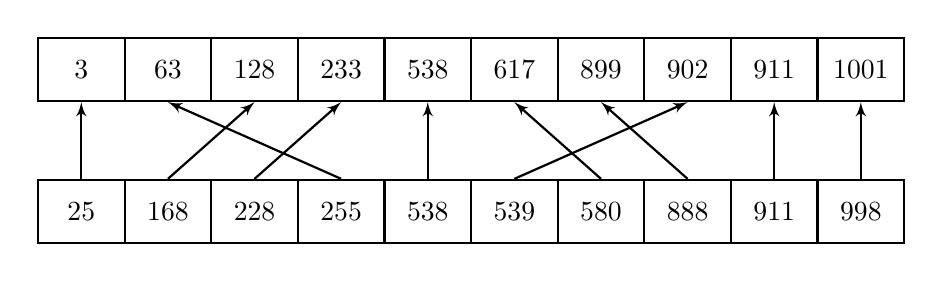
\begin{tikzpicture}[->,>=stealth',auto,
                 thick,node/.style={box, draw,font=\sffamily\Large\bfseries}]
                  \tikzstyle{line} = [draw, -latex']
                     \matrix (matrix) 
                     [
                         matrix of nodes,
                         row sep={1.1cm,between origins}, column sep=-\pgflinewidth,
                         row 1/.style={every node/.append style={myint}},
                         row 2/.style={every node/.append style={myint}},
                     ]
                     {
                        3  & 63  & 128 & 233 & 538 & 617 & 899 & 902 & 911 & 1001 \\[2em]
                        25 & 168 & 228 & 255 & 538 & 539 & 580 & 888 & 911 & 998  \\
                     };
                     \path [line] (matrix-2-1.north) --  (matrix-1-1.south);
                     \path [line] (matrix-2-2.north) --  (matrix-1-3.south);
                     \path [line] (matrix-2-3.north) --  (matrix-1-4.south);
                     \path [line] (matrix-2-4.north) --  (matrix-1-2.south);
                     \path [line] (matrix-2-5.north) --  (matrix-1-5.south);
                     \path [line] (matrix-2-6.north) --  (matrix-1-8.south);
                     \path [line] (matrix-2-7.north) --  (matrix-1-6.south);
                     \path [line] (matrix-2-8.north) --  (matrix-1-7.south);
                     \path [line] (matrix-2-9.north) --  (matrix-1-9.south);
                     \path [line] (matrix-2-10.north) -- (matrix-1-10.south);
               \end{tikzpicture}
               \caption{Illustration of the problem setting used, with the
               individual bitstring's phenotypic genes (lower array) sorted by
               value. The upper array shows the target integers, likewise sorted
               by value. The bitstring is evaluated by the sum of smallest pairwise 
               distances, with every gene linking to the integer in the target 
               set closest in integer-space, as long as no 
               other gene in the individual with a smaller distance to that specific
               target integer is present. The distance between the strings on the whole is evaluated as
               the sum of the distances. This particular example thus describes a total 
               distance of 673.}
               \label{fig:problem_description}
            \end{figure}

         In order to modify the complexity of the problem, i.e.\ to
         transform the search space, the measure of the total distance was passed 
         through four different functions of different styles,
         as described in \Cref{tab:complexity_functions} and visualized in
         \Cref{fig:complexities}. The cost function used to evaluate
         the individuals was chosen as the transformed distance.  
%
         %PUT TABLE AND FIGURE NEXT TO EACH OTHER? 

         \begin{table}[H]  
            \centering
            \caption{Transformation functions for changing the search landscape.
            All functions are defined $\forall x: x\geq0$, with the boundary
            condition that the function returns 0 at $x=0$.}
            \begin{tabular}{lm}
               \toprule            
               \textbf{Function name} & \textbf{Expression} \\
               \midrule
               Linear     & x \\[.8em]
               Stairs     & x - \displaystyle x \pmod{11} + \frac{11}{2}\\[.8em]
               Moguls     & x + \displaystyle 11\sin{\frac{x\pi}{11}} \\[.8em]
               Sharktooth & x + \displaystyle 22 \left|
               \sin{\frac{x\pi}{11}}\right|\\[.8em]
               \bottomrule
            \end{tabular}
            \label{tab:complexity_functions}
         \end{table}
            
         The \texttt{Stairs} modifier complicates the landscape by not allowing
         individuals to discern how far they are from the solution within the
         boundaries of the plateaus. The \texttt{Moguls} modifier, named after the bumpy
         trails in moguls skiing, instead complicates the search by alternatingly letting 
         individuals perceive the distance as closer respectively further from the 
         solution than it actually is. This implies that the hill-climbing abilities of 
         the algorithm are more important than in the \texttt{Linear} case. The
         \texttt{Sharktooth} modifier, again named because of the shape, is
         another take on the \texttt{Moguls} complexity, where the cost
         affiliated with evaluation is always greater than, or equal to, the
         non-modified distance.

     % * Reference software.

      \begin{figure}[H]
         \centering
         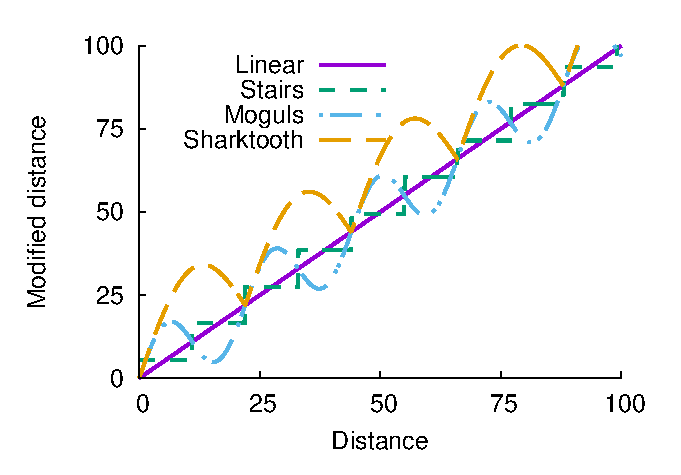
\includegraphics[scale=.9]{complexities} % loads
         \caption{Functions used to transform the search space of the GA. The
         mathematical expressions used can be found in
         \Cref{tab:complexity_functions}.}
         \label{fig:complexities}
      \end{figure}

   %ADD SOFTWARE FLOWSCHEME TO APPENDIX AND REFERENCE? 



\section{Results}
   \subsection{Analysing performance} 
   %% GRAY CODE SUPERIOR, BINARY MOST STABLE
   The Gray code scheme proved to in all of
   \Cref{fig:evol_trajectories}A-D be 
   superior in solving the designated objective. However, the average performance 
   varies significantly with the distance transformation
   functions, while the corresponding effect for the other encodings is not as
   noticeable. The Binary scheme is with respect to
   the different transformation functions the most stable, as it consistently
   ends up at roughly the same cost level in
   every complexity case. However, the only encoding whose performance noticably
   trends towards a slope of zero is the Gray code scheme, although the consensus sequences show
   tendencies to do so in the \texttt{Stairs} transformation as well. 
   %% GRAY CODE CAN'T OVERCOME BARRIERS

   %% CONSENSUS ENCODINGS TAKE ALTERNATE PATHWAYS, NON-CONSENSUS ALWAYS THE SAME
   Considering the error, it is also noted that the consensus
   encodings are affiliated with larger fluctuations than the
   bijective encodings in all cases. The consensus encodings are furthermore
   initially at a higher cost level than the bijective encodings. More precisely, 
   the Binary and Gray code schemes start with a cost of slightly less than 500, 
   while the consensus encodings begin just under 2500. 

   %% TIME
   The consensus sequences required a factor of 10 more computation time  
   to reach generation 100000, the consensus sequences took roughly an order of 
   magnitude more time to finish on average.
   The Gray code performed slightly worse than the Binary in the same analysis.

   For the consensus encodings, it is also noted that the cost level of the best
   individual in the population is improved by adding or removing start
   sequences in $90.6 \pm 1.3~\%$ of the cases for the Consensus Binary, as well as
   $90.0 \pm 1.5~\%$ for the Consensus Gray encoding.

   \begin{figure}[p]
      \hspace{-.5cm}
      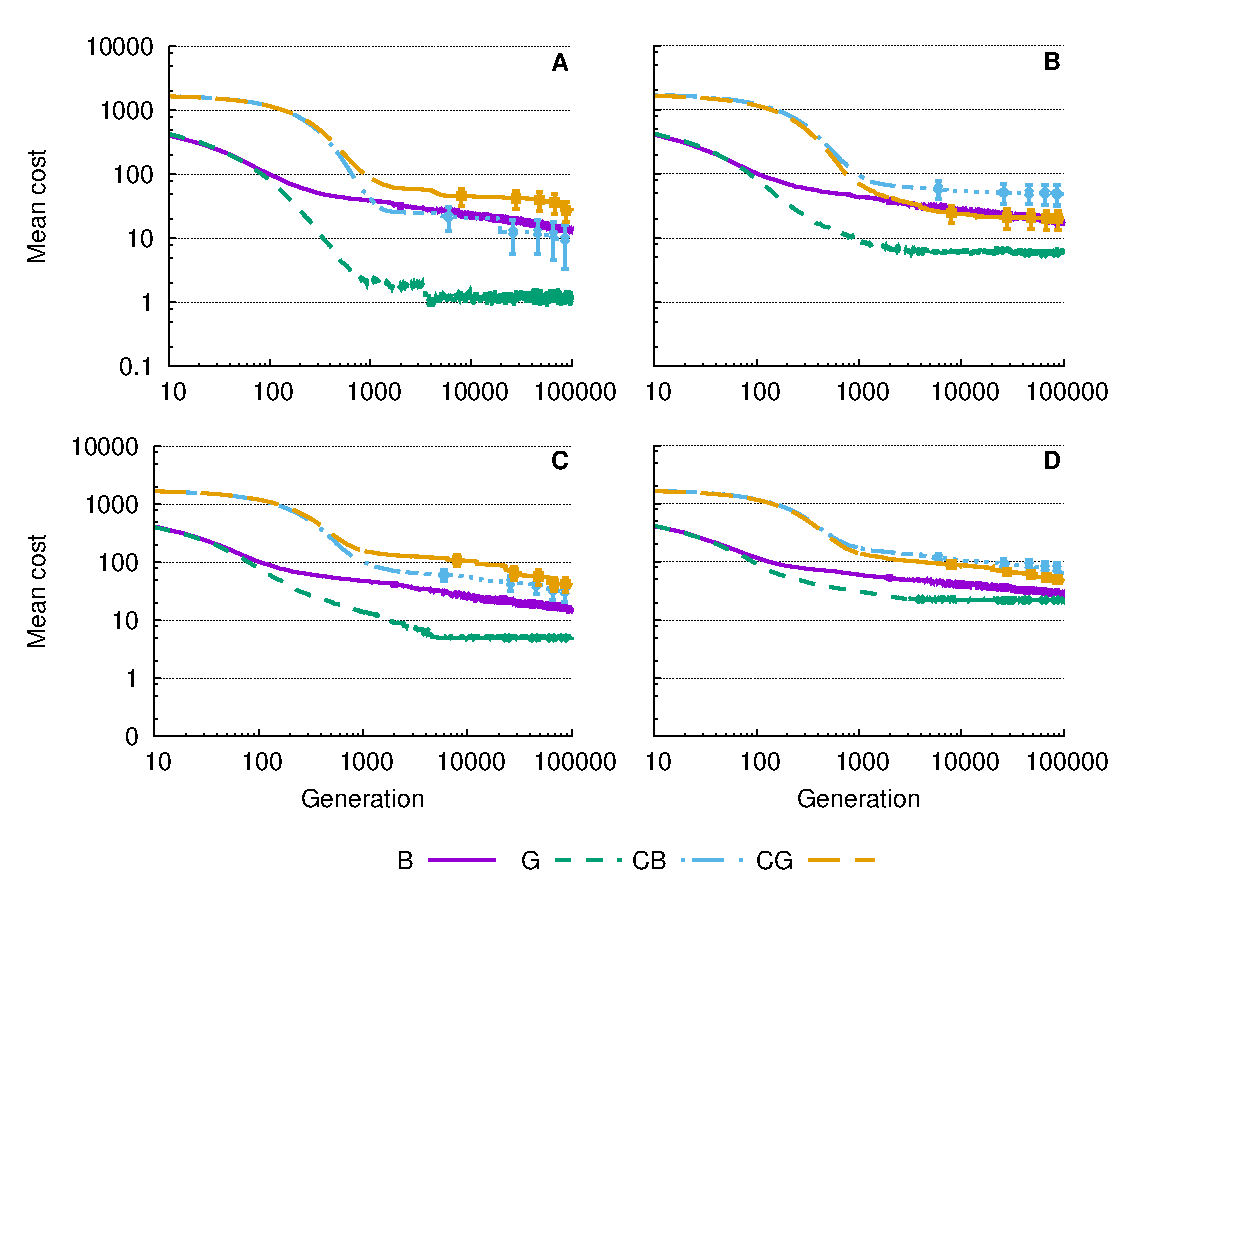
\includegraphics[trim=0 5.4cm 4cm 0,width=.9\textwidth]{multievoltest} % loads
      \caption{\textbf{A: Linear} \ \textbf{B: Stairs} \ \textbf{C:
      Moguls} \ \textbf{D: Sharktooth}\\
      Evolution of the mean cost trajectories for the four different transformation
      functions, sampled over 100 separate simulations, along with the  
      standard error of the mean. The cost for each separate simulation is given by the 
      transformed distance for the best individual in the corresponding population.
      }
      \label{fig:evol_trajectories}
   \end{figure}
  
   \newpage
   \subsection{Distribution of cost effects}
      %% BIJECTIVE VS NON-BIJECTIVE
      \Cref{fig:distribution}, which shows the distribution of cost effects
      at different cost levels, displays a clear distinction between the
      dynamics for the consensus and non-consensus 
      encodings. Due to parts of the genome not affecting the phenotype, 
      the amount of neutral mutations is higher in the non-bijective than in the 
      bijective cases, which is signified by the smaller areas enclosed by the
      curves. 
      Mutations on the consensus encodings also tend 
      to produce strings which have lesser negative effects, i.e.\ mutations
      which cause a higher cost, than mutations on
      the bijective encodings. In other words, the ratios for the bijective
      maps tend to evolve towards assuming a wider tail near the lower end of
      the range, whereas the same cannot be said for the consensus encodings. 
      Still, being more robust towards highly negative mutations does not imply
      having more positive effects. Instead, the bijective encodings 
      produce mutations which are positive to a larger extent than the
      non-bijective encodings. Furthermore, both consensus encodings do not 
      initially ($< 1000$) have the same distribution of cost effects, but 
      assume the same shape for lower cost levels, with minor deviations. 
      In observing the distribution of fitness effects by generation, as in
      \Cref{fig:distribution_generation}, the consensus sequences behave
      the same with respect to each other for each separate search space. This
      is even though the mean cost for the separate encodings often is
      different. 
      %% Bijective and non-bijective have different dynamics. How much is due to
      %% the averaging approach? 
      %% Non-bijective: less negative effects, not more positive effects. Due to
      %% averaging? Probably. Then why Gray code? I don't get it.
      %% Consensus have distribution effects corresponding to time rather than
      %% cost? 

      %% BINARY VS GRAY
      The bijective encodings behave similarly with respect to the shape of the
      distributions at different cost levels. The Gray code encoding produces
      slightly mildly negative effects more frequently, whereas the Binary encoding is 
      prone to produce more effects which are closer to the lower end of the range.  
      In most intervals and transformations, the Gray code scheme produces
      slightly more positive mutations, although largely such that the effects
      are only minorly positive. 

  %    %% CONSENSUS AND NON-CONS. BEHAVE DIFFERENTLY
  %    %% LIKELY DUE TO MORE NEUTRAL MUTATIONS

  %    %% LIKELY DUE TO ADOPTING A MORE GENE-ORIENTED STRATEGY
  %    All encodings tend to successively produce results which are of relatively
  %    more extreme nature, effectively shifting the distribution towards the lower
  %    end of the quotient spectrum, i.e.\ producing individuals which are relatively
  %    worse than the one undergoing the mutation.

  %    The lack of data in \Cref{fig:distribution}D stems from the fact
  %    that no simulations with neither the Binary nor the Consensus Gray schemes
  %    managed to produce individuals of the lowest cost level ($< 10$). 

   \pagebreak
   \begin{figure}[H]
      \vspace{-2cm}
      \hspace{-1cm}
      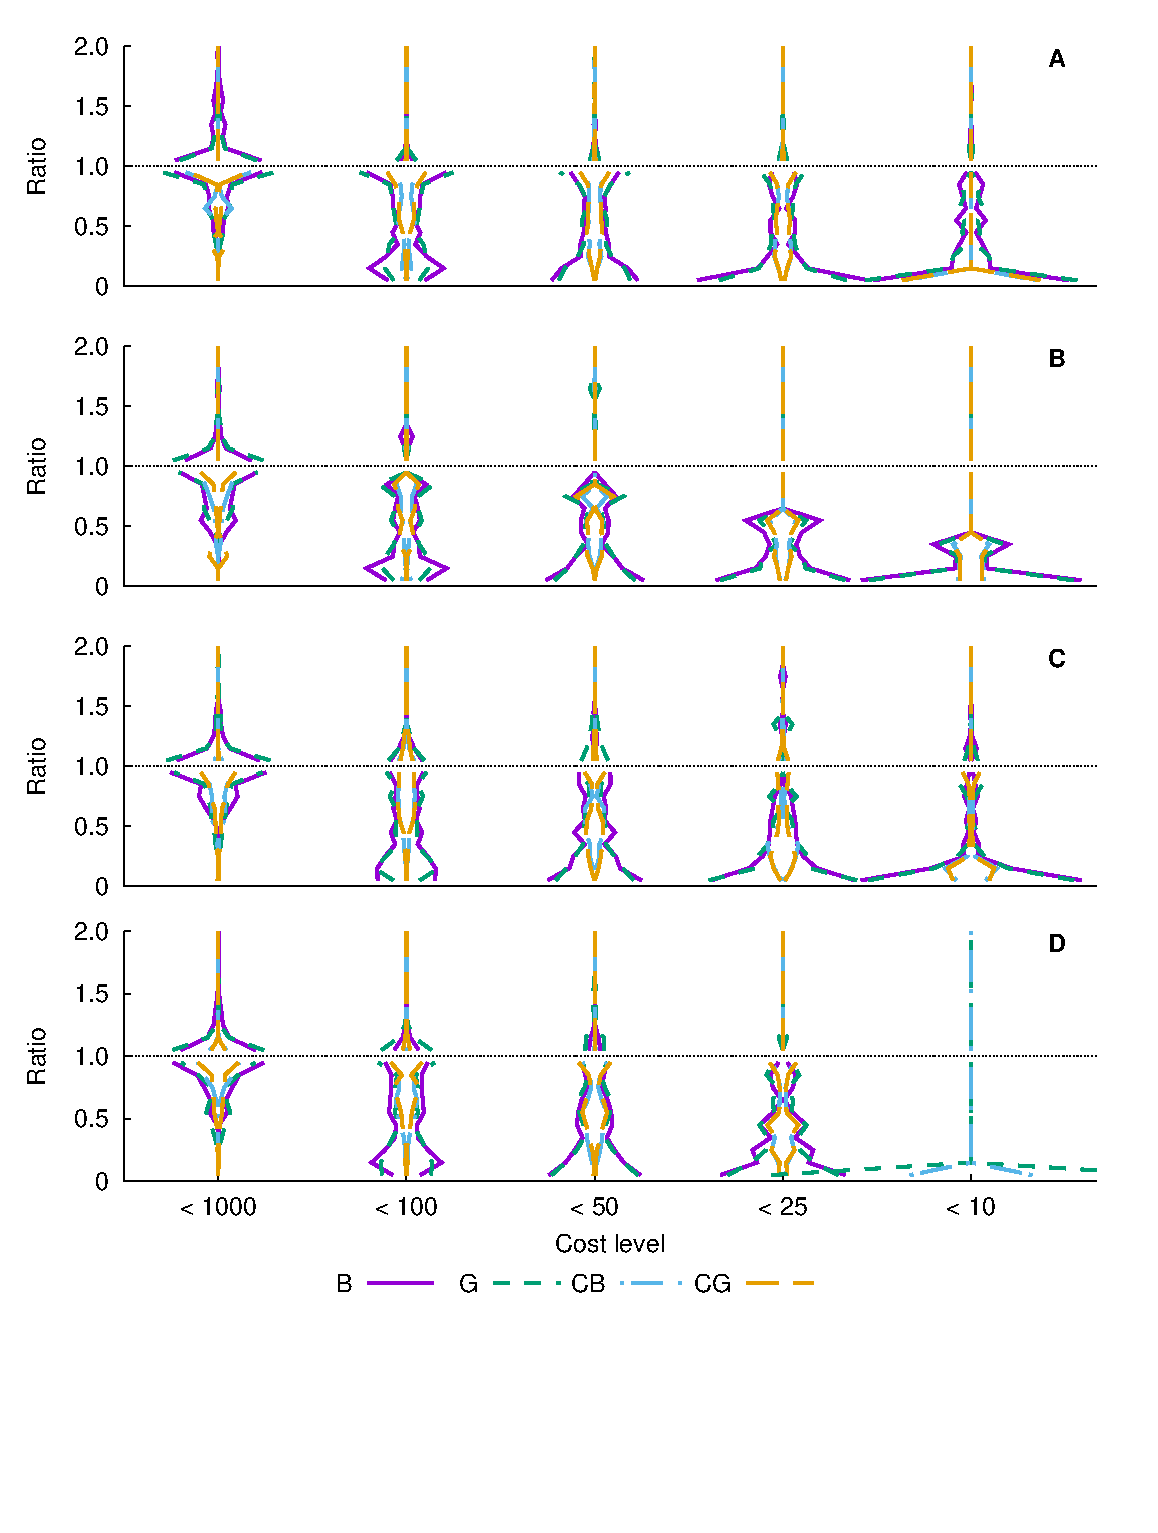
\includegraphics[trim=0 3.8cm 0 0,width=1.1\textwidth]{multihisto} % loads
      \captionsetup{width=1.\textwidth}
      \caption{
         \textbf{A:~Linear} \ \textbf{B:~Stairs} \ \textbf{C:~Moguls} \
         \textbf{D:~Sharktooth} \\
         \indent Distribution effects in binned intervals of
         0.1. The ratio denotes the cost of the individual before mutation,
         divided with the cost after.
         The inner horizontal axis gives the frequency
         of mutation effects for the corresponding ratio. All data are
         produced by mutating every individual with a parent from a higher
         cost level 10000 separate times, for a maximum of 100000 data points.
         Intervals do not overlap; for example, $\mathit{< 1000}$ signifies the
         interval $\left(100,1000\right]$. Neutral mutations as well as effects
         of magnitude $> 2$ are excluded in this figure. The lack of data in
         \textbf{D} stems from the fact that no simulations of the missing encodings manage to reach
   that cost level.}
      \label{fig:distribution}
   \end{figure}
   \pagebreak
      
   \subsection{Robustness to various mutation rates}
      Varying the mutation rate from the standard rate, as in
      \Cref{fig:multirobustness}, shows that the Binary and Gray code schemes 
      are more susceptible to higher mutation rates, whereas the consensus 
      encodings show significantly more robust traits. The consensus sequences
      contain a number of coding sequences correlating with the mutation rate,
      scaling from fewer coding sequences on average for higher ones, to
      more for lower ones (figure not included). 
      
      The Gray code scheme appears as to have a preference for lower
      mutation rates compared to all other encodings. In Figure 9C and D, it
      does however show a negative trend with a much lower mutation rate
      ($\times$1/10), as indicated by the slope of curve. The 
      slightly lower rate ($\times$1/2) performs on par with
      the standard rate in all cases, which is not the case for the Binary
      encoding. For the higher rates, both Binary and Gray perform equally bad. 

      The consensus sequences show tendencies to be biased toward a
      slightly higher mutation rate ($\times$2) in all of
      \Cref{fig:multirobustness}A-D. Even so, they manage to on average reach
      roughly the same cost level for all mutation rates. 

   \begin{figure}[p]
      \hspace{-.5cm}
      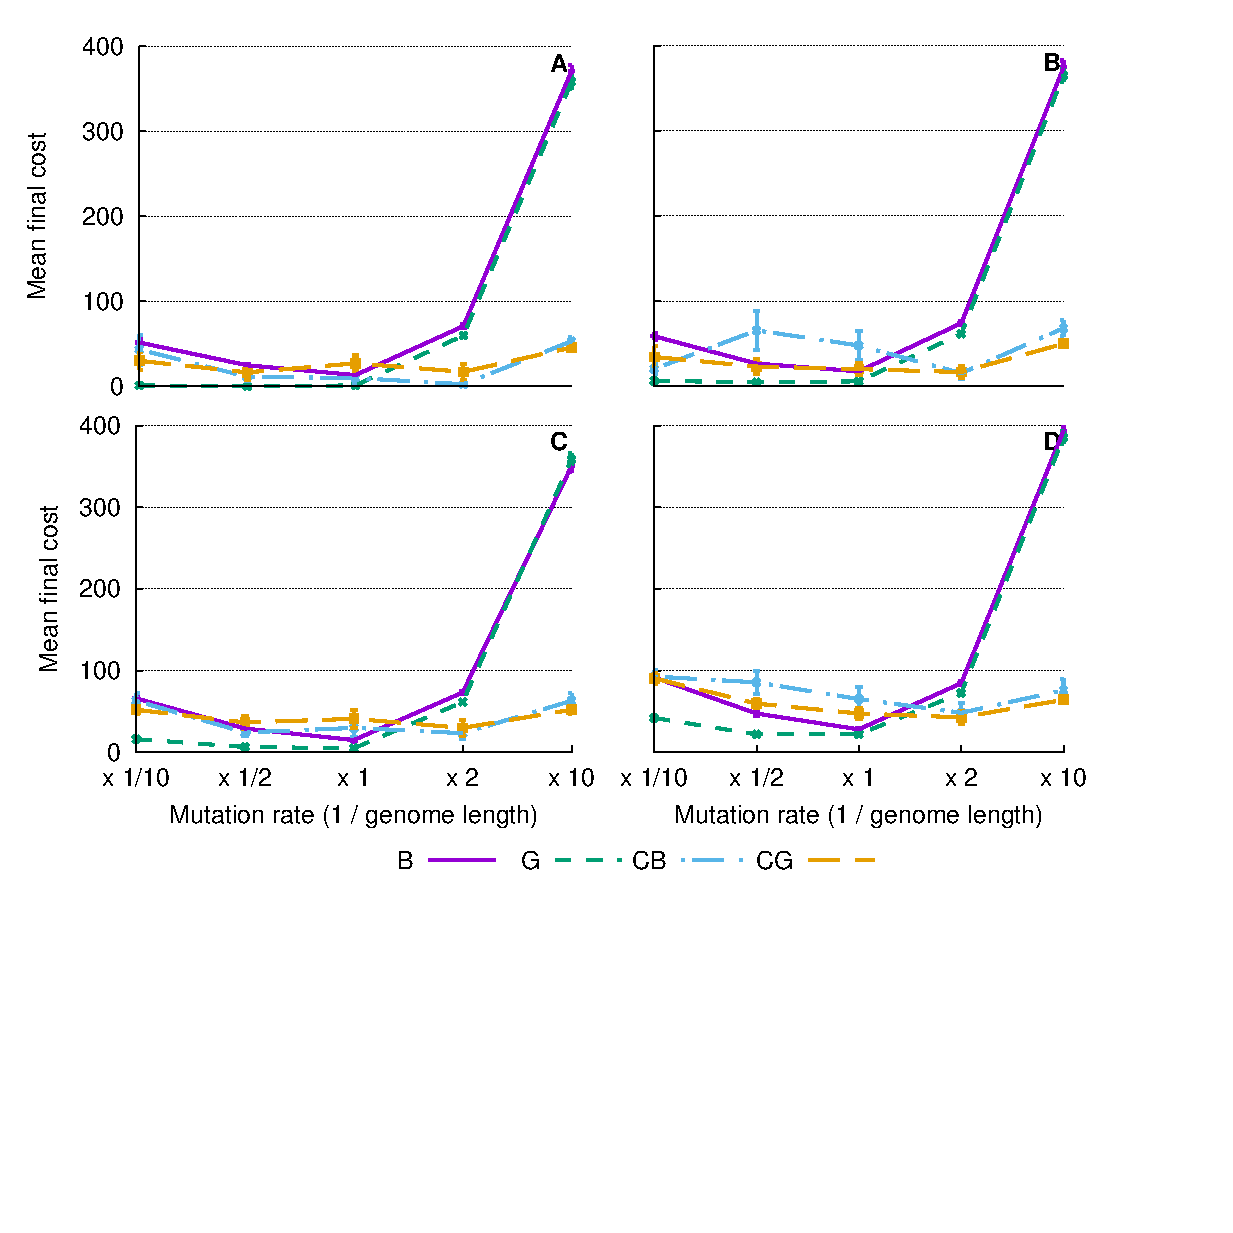
\includegraphics[trim=0 5.4cm 4cm 0,width=.9\textwidth]{multimutrates} % loads
      \caption{
         \textbf{A: Linear} \ \textbf{B: Stairs} \ \textbf{C:
         Moguls} \ \textbf{D: Sharktooth}\\
         Mean final cost values over 100 separate simulations per encoding. The mutation
         rate is modified by a given multiplicative factor (horizontal axis). Error
         bars show the standard error of the mean for the cost values at generation
         $100000$.
      }
      \label{fig:multirobustness}
   \end{figure}
      %% GRAY CODE MIGHT PERFORM BETTER, BUT EXTREMELY SUSCEPTIBLE

\newpage
\section{Discussion}
   \subsection{Evolution is determined by the accessible phenotypes}
      \subsubsection{Binary and Gray code encodings evolve by a different distribution
      of phenotype alterations}
      %% GRAY CODE SUPERIOR IN PERFORMANCE
      %It is likely that the Gray code gains its
      %superiority mainly from its inherent ability to take small steps in
      %phenotype-space, as well as its compact nature.
      %% GRAY IS THE BEST
      In comparing the different cases, a clear result is the superiority in the
      ability of the Gray code scheme to solve the problems given; it in
      particular fares significantly better than the consensus
      encodings, and in all but the \texttt{Sharktooth} transformation better
      than the Binary encoding. 
      %% BINARY MOST STABLE WRT COMPLEXITY 
      %% BINARY 
      In contrast to the Gray code scheme, the Binary scheme appears to get its strength 
      as an encoding primarily by being able to take larger steps in phenotype-space. As
      \Cref{fig:evol_trajectories} shows, when the search space changes under the
      different transformations, the Binary code performs qualitatively
      the same in most cases, but with a slightly higher mean cost in 
      \Cref{fig:evol_trajectories}D. This indicates that the
      Binary encoding is able of overcoming the induced barriers mainly by taking large
      steps in phenotype space in all cases. 
      
    %  In the two cases which are especially hard for the Binary encoding, i.e.\ the 
    %  \texttt{Stairs} and \texttt{Sharktooth} case, the transformed search space functions as a barrier
    %  which occasionally either is too great for the Binary scheme to overcome,
    %  or requires phenotypes which are not easy to reach. 
    %  
    %  The sharp minima, as seen in
    %  \Cref{fig:complexities}, creates a higher pressure for the population to be
    %  centered around those points than in the smooth case of the
    %  \texttt{Moguls} space, and subsequently limits the accessible states. 
    %  Because the Binary encoding 
     
      %% GRAY CODE
      %% Other ss remove benefit of Gray as more complex mutations are needed.
      For all but the \texttt{Linear} transformation, the landscapes appear to in
      various degrees remove the benefit of the Gray code scheme, i.e.\ not
      having Hamming cliffs,
      as it struggles with the altered complexities. However, the Gray code scheme is like
      the Binary encoding able to perform large translations in phenotype-space
      as well, which makes it probable that the reason for the Gray code 
      outperforming the Binary scheme is the ability to take \textit{both} small
      and large steps, whereas the Binary has a more rigid distribution of possible
      steps. When the search spaces are transformed in especially
      \Cref{fig:evol_trajectories}C and D, an advancement in cost requires
      larger changes in the phenotype to overcome the induced barriers, which
      explains why the Gray code scheme is somewhat hampered -- the
      importance of being able to make small phenotype changes is reduced. 
      Still, being able to take smaller steps which do not have
      drastically negative consequences, i.e.\ having near-neutral mutations, allows the
      population to spread out near the current local optimum to a larger extent
      than for the Binary scheme. As taking both small and
      large steps is a significant separator of the Gray code from the Binary,
      it is an important factor for the Gray code producing better results.  
      
      % Neutral mutations, random walks, single bit flips vs. ultiple
      \Cref{fig:multirobustness} shows that the Gray code scheme generally
      performs equally well with a slightly lower mutation rate ($\times$1/2)
      as with the standard one. This indicates that the scheme primarily evolves by
      manipulating single bases, which would explain the Gray code encoding being able to 
      outperform the Binary in the \texttt{Stairs} transformed 
      search space, which effectively forces the bijective encodings into having
      neutral mutations also when the genotype is affected. 
      In particular, this shows the significance of neutral mutations in a
      somewhat unexpected sense; the Gray code encoding being able to 
      perform a cost neutral random walk in the vicinity of the current state gives it a higher
      probability of reaching a better optimum. In other words, the Gray coded 
      strings can then effectively random walk until a
      state from which a translation to a lower plateau is reached. 
      The Binary scheme would in principle be able to do the same, but is because of its
      design hampered with respect to what adjacent states are reachable from the current
      one, i.e.\ the Binary scheme is unable to randomly walk within the vicinity of the 
      current state as proficiently as the Gray code scheme. It instead relies
      more on multiple bit flips in order to attain desired states. The dynamics
      of the encodings can be emphasised further inspection of~\cref{fig:distribution},
      where the Binary and the Gray code schemes have very similar distributions with
      respect to the cost effects. Regardless of this, the Gray code performs better,
      indicating that it is not solely the distribution of possible jumps that
      is important, but also the connection between states. 

      %% Significance of coupled mutations -- neutral mutations
     
     %%%%%%%%%%%%%%%%%%%% 
      \subsubsection{Consensus encodings evolve by adding and removing random numbers}
%      Likewise, the consensus encodings are, independently of the method
%      to interpret the coding sequences, unable to take sufficiently large steps
%      in phenotype space, which is the reason for them not being able to evolve
%      as well as the bijective encodings.
      
      %% CONSENSUS ENCODINGS FLUCTUATE MORE -- ALTERNATE PATHWAYS
   %   The consensus encodings are also affiliated with significantly larger
   %   fluctuations, indicating precisely what was found by Shipman et al.\ 
   %   \cite{Shipman2000} -- that neutral encodings allow for alternative
   %   pathways. As the Binary and Gray code schemes are not associated with larger
   %   fluctuations, it is reasonable to assume that they have
   %   identical or largely similar approaches between the separate simulations,
   %   e.g.\ mutating the bits of each individual number independently, without
   %   any cross-interaction between the genes, such as interchanging mappings after
   %   mutations. 

      %% EVOLVE EVOLVABILITY
      The consensus encodings behave similarly under all search space
      transformations in that they all take about the same number of generations before starting to
      effectively decrease in cost. This indicates that the consensus sequences have a 
      tendency to evolve \textit{evolvability}, and that two things are
      likely needed to be balanced: 1) the number of coding sequences, and 2) the
      relative difference between the coding values. As these two points determine the
      available translations in phenotype-space that the individuals are able to
      undergo, it is a significant factor for the ability to improve. 

      %% CONSENSUS ENC. ARE EXTREMELY SIMILAR
      To expand on this, the consensus encodings do not show significant enough differences
      in performance. Instead, the reason for their ability to evolve and solve the
      problem seems to depend on their inherent structure, i.e.\ by being able
      to average over a set of coding sequences. As the evolution is mostly
      governed by the destruction and creation of coding sequences, the
      phenotype alterations essentially consist of adding and removing
      quasi-random numbers. 

      In principle, the consensus sequences should be able to
      perform both small and large jumps in phenotype space directly by their
      structure by either manipulating the coding bases to cause a significant change
      within the separate coding sequence (larger translations in integer-space),
      or by modifying moderately-valued bases (shorter translations). 
      In practice, however, the consensus encodings do not have close access to the appropriate
      phenotypes, and thus fail to perform on par with the Gray code scheme. They can also not, due to the
      averaging of the coding sequences, take as large steps as their
      bijective counterparts, which could be a limiting factor for their ability
      to evolve. In particular, because the random numbers which can be
      generated by introducing respectively destroying coding sequences depend
      on the current state, the consensus sequences are like the Binary encoded
      strings limited in what phenotypes are possible to be obtained practically. The low probability of
      inverting any of the coding bits required to drive the evolution 
      makes it too hard for the consensus encodings to competently evolve, even
      though they in principle can assume all phenotypes the bijective encodings
      can assume, in multiple ways.
      
      %% CONSENSUS ENCODINGS HAVE ALTERNATIVE INITIAL POINTS. DUE TO (ONE) TWO THINGS
      %% RANDOM INITIALIZATION DISFAVORS CONSENSUS THE AVERAGING IN CONSENSUS ENC
      Finally, that the consensus encodings have trajectories which have a
      higher initial cost (see \Cref{fig:evol_trajectories}) is due to many 
      genes being initialized with multiple coding sequences,
      so that the phenotypic value of the genes average at around $1023/2 
      \approx 512$. With a genome length of 1000 bits as well as a start
      sequence length of six bits, a start sequence can be estimated to occur on
      average roughly once per $(1/2)^{-6}$ bases. Accounting for sequences not being
      allowed to overlap, as well as the length of the coding sequences themselves,
      gives an estimate of roughly 12 start sequences per gene. Because of this,
      the initial cost of the consensus sequences is as high as it is. 

   \subsection{Small differences in the distribution of mutation effects cause significant
      differences in performance}
      From the distributions seen in \Cref{fig:distribution}, although the Binary and Gray 
      code schemes initially behave differently, they ultimately assume roughly the same behaviour.
      However, even though the distributions show small differences between the
      Gray code and the Binary schemes, the encodings still perform significantly
      differently from each other.
      The amount of neutral mutations on the individuals can also be seen in the
      difference in the area under the curve between the bijective and
      non-bijective encodings. 
      
      When the Gray code and Binary schemes
      nonetheless do ultimately perform roughly similar to each other, as in
      \Cref{fig:distribution}D, the Gray code can still be seen to
      consistently produce mutations with better results than the Binary scheme, 
      indicating that the Gray coded strings are the only ones undergoing significant
      improvement at that cost level. Even so, also the Binary consensus encoding
      manages to reach the lowest cost level ($< 10$), even though no
      significant positive mutation effects are visible in the next-to-lowest cost 
      level. 

      %% CONSENSUS SEQUENCES HAVE NEUTRAL MUTATIONS
   \subsection{The consensus structure allows for higher robustness}
      Consensus sequences are clearly favoured with respect to their
      ability to evolve under various mutation rates. Especially under high
      rates, both the bijective encodings fare far worse, whereas the
      consensus encodings appear to be biased towards a slightly higher mutation
      rate.  
      The bias is likely due to consensus encodings having a proportionally lower amount 
      of bases which individually affect the phenotype. They therefore
      require a slightly higher mutation rate to invert significant bits;
      however, as the mutation rate stands in relation to the genome length,
      the slightly higher rate ($\times$2) for the consensus sequences
      corresponds to a sub-standard mutation rate for the bijective maps. 

      Because of the averaging approach, if many genes are present,
      not only are individual inversions of bits less significant, but the least
      significant bits in each coding sequence become redundant. It is also
      because of this approach, i.e.\ the collaboration between coding
      sequences, that the consensus sequences are able to adapt.  
      
      %However, the consensus encodings are thereby still able to adapt enough to produce
      %relatively good results also at low mutation rates, which appears to be
      %problematic for especially the Binary encoding.  

   %  ROBUSTNESS
      %% GRAY CODE PERFORMS BETTER, BUT SUSCEPTIBLE TO HIGHER MUTATION RATES
      %% CONSENSUS ENCODINGS MORE STABLE ON THE WHOLE, BOTH TOWARDS LOWER &
      %% HIGHER RATES   
   %  COMMON
      %% COMPUTATIONALLY: CONSENSUS ENCODINGS SLOW, BUT COOL TRAITS
\section{Concluding remarks}
   It has here been shown that the choice of encoding further plays an important
   role for the performance of GAs. In agreement with previous statements,
   bijective maps seem favourable in many cases, as the Gray code scheme comes
   out as superior in performance in all investigations when the mutation rate
   is set to unity of the genome length or slightly less. However, that the
   consensus encodings manage to produce results on par with the Binary encoding
   signifies that bijectivity is not the sole aspect of choosing an encoding.
   Instead, \textit{how} the search space is traversed, and what types of
   translations in phenotype-space can be performed by the encoding is also of
   essence. That the Gray code scheme comes out so superior seems to be
   because of its ability to take both smaller and larger jumps in this space,
   and in particular because of being able to access adjacent phenotypes.
   Introducing an encoding which is able to do so with another distribution
   of accessible states depending on the current one might be a possible topic 
   for future research. 
      
   It has also been noted that the consensus sequences produce more stable results under
   different mutation rates than the bijective encodings, which emphasises their adaptive 
   structure. The Gray code and Binary schemes are, because of their bijectivity 
   intrinsically unable to adapt to environments with higher, and presumably 
   also lower, mutation rates. The dynamic structure of the consensus encodings makes 
   the consensus encodings more flexible, and therefore possibly better in changing
   environments. 

   The analysis has shed further light on the dynamics
   of both bijective and non-bijective encodings, as well as their similarities
   and differences. Hopefully, this can be used to broaden 
   the understanding of the deep complexity of GAs, but also of evolutionary dynamics 
   in general. 

\section*{Acknowledgments}
   Many thanks to my main supervisor, Carl Troein, who gave me such great
   independence with my project, and who showed me that details do matter --
   sometimes the most. I am also
   grateful for Klara Berg, to whom I could always talk to about anything. Also my office 
   colleagues deserve a mention for the many inspiring and interesting discussions had 
   during the course of the project; in particular Frank Johansson and Mårten Bertenstam, 
   thank you. However, my greatest gratitude belongs to Adriaan Merlevede, who was 
   always there, and prevented me from trying to fly too high. Oh, and thank you, 
   Julian Melgar -- thank you!
   
%\section*{Acknowledgments}
%%   Farväl till allt. 
%   I would like to thank my main supervisor, Carl Troein for giving me such great
%   independence in working with this project, and for showing me that details
%   \textit{do} matter -- perhaps the most. I am also grateful for Adriaan
%   Merlevede, who taught me the importance of realistic expectations and
%   prevented me from turning into an Ikaros story. Lastly, I am the most
%   thankful to Klara Berg, who always was there. Oh, and thank you, Julian
%   Melgar -- thank you!
   
   \newpage
\appendix
\section{Appendix}
\subsection{Distribution of cost effects by generation}
  % \subsection{Wordlist}
  %    \paragraph{Genotype}
  %    \paragraph{Phenotype}
  %    \paragraph{Fitness/Cost/Objective function}
  %    \paragraph{Encoding}
  %    \paragraph{Bitstring}
  %    \paragraph{Population}
  %    \paragraph{Genetic Algorithm}

   \begin{figure}[H]
      \vspace{-.5cm}
      \hspace{-0cm}
      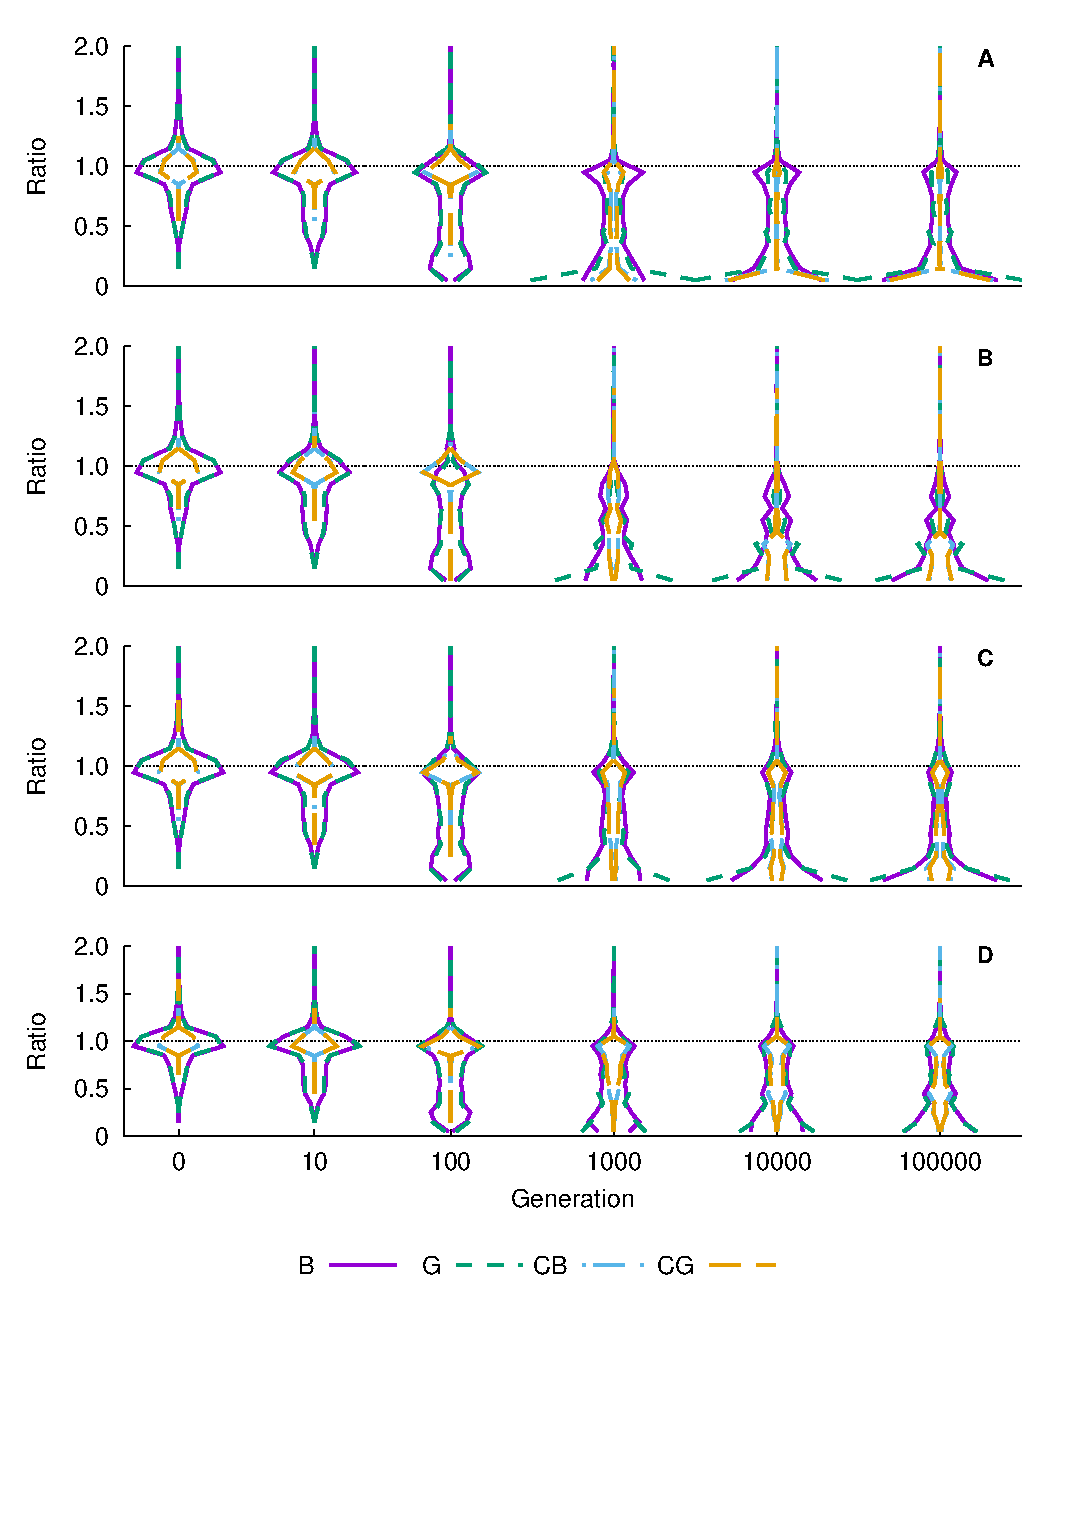
\includegraphics[trim=0 4.7cm 0
      0,width=1\textwidth]{multihisto_generation} % loads
      \captionsetup{width=1.\textwidth}
      \caption{
         \textbf{A:~Linear} \ \textbf{B:~Stairs} \ \textbf{C:~Moguls} \
         \textbf{D:~Sharktooth} \\
      \indent Violin plot analogous to \Cref{fig:distribution}, but with
      the mutation effects given by generation. }
      \label{fig:distribution_generation}
   \end{figure}

 %     Notably, a common trait with respect to the dynamics of the mutation
 %     effects, seen in \Cref{fig:distribution}, is that all encodings feature a
 %     similar flow of frequency, as the amount of near-neutral mutations
 %     decrease in time to favor
 %     the prevalence of mutations that perform negatively. However, it is important 
 %     to note that the mutation effects stand in relation to the current
 %     fitness, and as the encodings perform differently, this has to be
 %     considered. 

 %     Regardless, one can note that the distribution of fitness effects behaves
 %     equivalently between the encodings aside from the fact that the consensus
 %     schemes allow for neutral mutations to a wider extent, as can
 %     approximately, due to the cutoff, be seen visually as the difference in
 %     enclosed area. 
 %     
 %     The tendency of converging is visible in the amount of mutations giving
 %     rise to a quotient value of 0, as it indicates that the mutated
 %     individuals are infinitely worse than the previous one. Especially in
 %     \Cref{fig:distribution}D this can be noted, as the mutations on the
 %     consensus encodings still have not reached the solution to a significant
 %     enough degree for any results to show up in the distribution.  
\printbibliography
\newpage
\end{document}

